\addtocontents{toc}{\cftpagenumbersoff{chapter}}

\setstretch{1.5}

\chapter[INTRODUCTION]{\fontsize{16}{12}\selectfont INTRODUCTION}

\pagenumbering{arabic}

\section[Background]{\fontsize{14}{12}\selectfont \MakeUppercase{BACKGROUND}}
RFId (Radio-Frequency Identification) is a technology that allows remote recognition of an item by means of radio communications. A transponder (also named tag) is coupled to the object that one has to recognize. The tag can record information such as personal data, photos, bar codes, Id codes, date and time of a transit, direction of the transit, and other information. 
The tag can be printed or inserted into objects of different shape (such as a badge), and coated with the most suitable material for the usage that one wishes to do and then customized with prints, images, texts, logos, photos and bar codes. A suitable reader interrogates the tags to obtain the information of interest. Before using an RFId system as part of a control system for a safety application, one has to know the way the RFId system operates and understand the best way to use it.

\begin{comment}
\begin{figure}[h!]
	\centering
	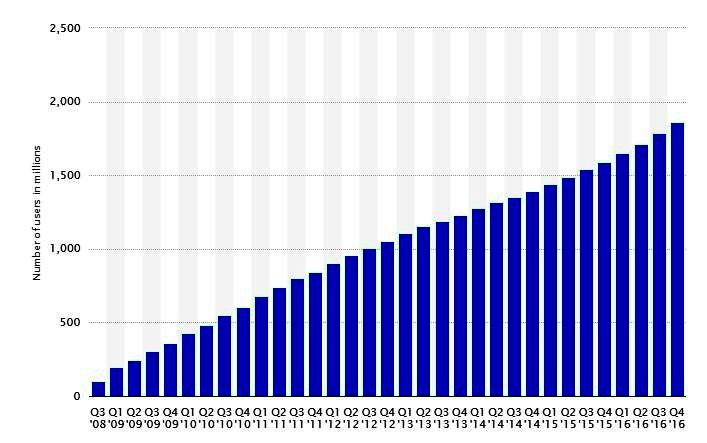
\includegraphics[scale=0.7]{fb.jpg}
	\caption[Number of Monthly Active Facebook Users World wide as of 4th Quarter 2016 (in millions)]{ Number of monthly active facebook users worldwide as of 4th quarter 2016 (in millions)}
	\label{fg}
\end{figure}
\end{comment}

\addtocontents{toc}{\cftpagenumberson{chapter}}

\chapter[LITERATURE REVIEW]{\fontsize{16}{12}\selectfont LITERATURE REVIEW}

\section[USAGES IN MACHINERY APPLICATIONS]{\fontsize{14}{12}\selectfont USAGES IN MACHINERY APPLICATIONS}

\subsection[Usage in machinery safety applications]{Usage in machinery safety applications}

An RFId system cannot be used as an ESPE (Electro sensitive protective equipment). Such equipment is used in a control system of a machine to prevent access to dangerous areas. The device operates when an optical beam is interrupted by the passage of objects or parts of the body of a person. In practice, the instant the beam is interrupted, the control system knows the position of the person who is interrupting it. In the time interval that precedes this event the control system assumes that there is no dangerous situation, yet there is a non-zero probability that in the time interval that comes after the interruption a dangerous situation could be present, for such reason the control system initiates actions that bring the machine to a safe state. 

\vspace*{1pc}
An RFId system cannot know the position of anything that has not been previously associated with a tag (it recognizes the presence of tags within its operational area). For such a reason it can’t put the machine in a safety state if any subject without a tag enters the operational area of the reader. Actually, the system could be able to initiate an action only if people who wear a tag come into this area. Such behavior is not safe in an ESPE.  

\vspace*{1pc}
Conversely an RFId system works very well to permit access to a hazardous area to persons who are authorized (i.e. provided with an authorized tag), then an RFId system works very well as key, or to allow the activation of certain devices (e.g.: work equipment) only by a known operator (with tags). In fact, from this point of view it has even higher functionality, as the tag is associated with an identifier, fact this that allows the implementation of a hierarchy of permissions.

\vspace*{1pc}
As an example, some individuals may be allowed to access certain areas and others to different areas, or some subjects can unlock some operation modes of the work equipment, such as the "maintenance mode", and other people can’t, and so on. In practice, in many applications one can’t use the RFId system as the main safety issue, because it only protects those people who wear a tag, but one could use it as an additional safety device. Without doubts it is easier (and natural) its use as a "key" or as a tool to disable a safety barrier, or to access to a particular operating mode (e.g. "maintenance mode", "training mode").

\subsection[Usage as additional safety device]{Usage as additional safety device}

In some cases, it is conceivable that the operation of a tool or equipment is allowed only in presence of operators (e.g.: a press or a CT scan or other). Such equipment may require special procedures to ensure the safety of people, by preventing unauthorized use or by stopping operations if there isn’t an authorized operator in the work area. During maintenance or other operations (for example: training) equipment can be operated, often in controlled mode (for example with a lower speed or with a reduced power). 

\vspace*{1pc}
But even in controlled mode there may be a residual risk which is not negligible, especially when there are third persons approaching the danger zone, that usually have nothing to do with the work going on. When such situations arise it can be in favor of safety if the operation, possibly in a controlled mode, can only be activated when the personnel authorized to operate in that particular mode (the maintainer, the trainer), provided with a tag, is present near the equipment. 

\vspace*{1pc}
To return to normal operation, however, it is better to be sure that the personnel, that before was in the hazardous area, be at the right distance from the hazardous parts (safety lock that can only be disabled when the reader no longer detects the tags inside its operational area). 

\vspace*{1pc}
Note that, in this case, the RFId system behaves as an additional protection (in fact it is not capable of detecting the presence or absence of persons not equipped with tags), this should not exempt anybody from the use of interlocks or shelters that can be opened only with a tool and a voluntary consent for the reactivation of the normal operation of the work equipment. 

\subsection[Usage as safety interlocking device]{Usage as safety interlocking device}
The interlocking devices of shelters of machinery are constituted by a position switch and an actuator that, at the opening of the shelter, actuates the position switch. The ISO 14119 standard classifies them into 4 types. Type 4 interlocking device, "interlocking device with non-contact actuated position switch with coded actuator", is able to operate with magnetic actuators, RFId tags or optic actuators.

\vspace*{1pc}
In this case the RFId system constitutes the actuator of the position switch when the shelter is closed. The advantage in the use of RFId systems is due to the fact that they are resistant to shocks and vibrations and allow high alignment tolerances. 

\subsection[Usage as an additional PPE]{Usage as an additional PPE}
An RFId system can be used to lock the operation of equipment in the event of the fall of an operator through openings beyond which there are moving parts. This is the case, for example, of threshing machines, harvesters, water pumps, shaving machines. In such equipment hay, grasses, liquid substances, wood enter from an input opening during normal operation. However, if the accidental entry of an operator happens then it is necessary to stop the moving parts. 

\vspace*{1pc}
In order to timely protect operators one can use an RFId system. The passive tags are integrated on the clothing or on bands that can be worn at the limbs, in the trunk/hips area, in the head/neck area, while the reader is placed at the input opening which must be located sufficiently distant from the moving parts (the operational area of the reader coincides with the input opening area). 
Unfortunately, a similar equipment is not a main safety related part of the machine but only an additional PPE, in fact it has the disadvantage of protecting only operators who wear tags and not any other person. 

\section[USAGES IN WORKPLACES]{\fontsize{14}{12}\selectfont USAGES IN WORKPLACES}

\subsection[Usage as an access key to a building site]{Usage as an access key to a building site}
An RFId system can be used to allow access to a building site only to the personnel who wear the prescribed PPE, for example by integrating appropriate passive tags on every item of PPE and positioning at the entrance of the site a reader, so that access is possible only to those subjects that wear all the necessary PPE. The same can be applied if the site is divided into zones and in each zone there is a specific requirement for the provision of PPE: in fact, the reader at the entrance to each zone can determine if one wears all the necessary PPE to allow his/her admission to that particular area. 

\vspace*{1pc}
It is possible that the tags associated with the same type of PPE have the same identification code, however, given the versatility of RFId systems, it is possible that each PPE has a unique identification code, which allows to associate it exclusively to a single owner. In this case it is possible to know moment by moment who is located within a specific area and if he/she is wearing the provided PPE. 

\vspace*{1pc}
Some work equipment (with reader) could be made unable to activate if the operator does not have special permissions and/or if he/she does not wear specific PPE. The check, that can be made by the RFId management system (through the activation of an appropriate application), is based on the fact that each worn PPE (equipped with a unique tag) is exclusive to a specific operator. 

\vspace*{1pc}
Moreover, it is possible that a portable terminal (mobile phone, tablet, Personal Digital Assistant) be able to carry both the reader feature, for passive tags associated with the PPE (the terminal, permanently worn by the person who is protected by the PPE, can warn the worker if he forgets or loses a particular PPE), and the active tag feature, for a three-dimensional localization system of workers within the site.

\subsection[Usage for localization of workers]{Usage for localization of workers} 
An RFId system is a viable alternative to both the traditional personal identification technology (badges, etc.), and to the biometric technology based on the recognition of individual attributes. Unlike these technologies it also allows the "distance" recognition. The identification through RFId tags permits ways of distinguishing between inputs and outputs, and automatically checks the attendance list in a given area. Moreover, as seen, it allows the startup or shutdown of devices depending on the fact that the authorized operator is nearby. 

\vspace*{1pc}
An RFId system using active tags can be used to achieve a three-dimensional localization function of workers within the workplace (in the presence of at least four readers positioned so as not to lie all on the same plane). The three-dimensional localization system can be useful to facilitate the emergency operations, for example the localization of a worker during the exodus phases. This function is made possible by the existence of a historical database of worker positions, which allows to look for the missing worker at his/her last recorded position. 

\section[USAGE AS A SAFETY INVENTORY]{\fontsize{14}{12}\selectfont USAGE AS A SAFETY INVENTORY}
 
An application of an RFId system may be the location of a tool, a work equipment or a container of a substance, with particular regard to tools, equipment and substances whose location could have consequences on safety (for example, hazardous tools, equipment and substances). This can be achieved by placing a tag on the tool, on the equipment or on the container of the substance and making sure that a reader controls the access to the chosen location place. 

\vspace*{1pc}
The typical application is the control of the tool inventory at the end of work, which can also occur during off-site working operations or during operations for which a similar control is important (or necessary for economic reasons).  

\vspace*{1pc}
The reader can signal after work if a tool wasn’t placed back (it can also indicate which one, thanks to the tag identifier). Eventually a portable reader can be passed onto the work area or in its vicinity, to find missing tools. 

\vspace*{1pc}
Such a system does not allow, when used in relation to tools, equipment or dangerous substances, to avoid the simultaneous adoption of quality procedures for tracking, however, it can serve the purpose of making the accomplishment of inventory operations considerably faster. 

\vspace*{1pc}
The RFId system is also useful in reconstructing the history of the tool, of the work equipment or of the container, since, thanks to a database that is updated on the basis of the data received from the reader, one can obtain information about usage, maintenance and verification (and contained substances in the case of the container), which can then be sent on the terminal (mobile phone, tablet, Personal Digital Assistant) of the worker that uses the tool, the equipment or the container (the terminal can be provided with RFId, label or q-code readers). 

\vspace*{1pc}
It is interesting the application of RFId systems to the maintenance of chemical plants, where information about the maintenance of the valves have considerable importance. With a simple reading of the tag of a specific valve, it may be possible to get in few moments the entire history of maintenance and repairs of that valve.
 
\section[USAGE FOR ENVIRONMENTAL PARAMETERS RECORDING]{\fontsize{14}{12}\selectfont USAGE FOR ENVIRONMENTAL PARAMETERS RECORDING} 
A particular application of RFId systems relates to the use of active tags equipped with sensors able to detect climate parameters (temperature, pressure, humidity) of the environment in which they are immersed. The measured parameters are stored in an internal memory, until it is downloaded by an operator, thanks to a reader. 

\vspace*{1pc}
In specific industries where it is necessary to ensure controlled operating schemes for the environment, a tag, thanks to its small size, can be placed in the uncomfortable points of the equipment, where it is difficult to bring the cable needed to supply a measuring device and offer, at content costs, a reliable and easily achievable solution. 

\vspace*{1pc}
For example, an application related to the cold chain is to control and maintain a proper temperature during the phases of distribution (transportation, storage, delivery and allocation) until the time of retail, in order to ensure integrity and quality of products. 

\vspace*{1pc}
The tags for this application incorporate a temperature sensor. There are two types of sensors: the first type records the peak temperature or the occurrence of an exit from a predefined temperature range, the second type, instead, operates in a continuous way, by monitoring the temperature in time. Even for sensors that operate in a continuous manner it is possible to program the measuring temperature range and store the values, so as to obtain a graph in time or identifying the instant in which there was the exit from the predetermined temperature range. 

\vspace*{1pc}
Through the use of such systems one can monitor the conservation status of a substance/product without opening the packages. Hence it is possible the management of data by computer, by taking the necessary decisions centrally, such as the elimination of the product, or the application of a treatment, or other. 

\vspace*{1pc}
The type of sensor used and the amount of memory required can affect the cost of the tag. Moreover, since the specific tag is a costly item, then, for not losing it, it is also necessary to evaluate the cost for the return logistics. 

\section[USAGE AS A SOLUTION FOR INSTALLATIONS]{\fontsize{14}{12}\selectfont USAGE AS A SOLUTION FOR INSTALLATIONS}
In medical rooms, but also in workshops or other work environments, it may occur that supply systems with different characteristics are needed within the same local, to feed users who require a specific supply.

\vspace*{1pc} 
There are multiple solutions to be sure that the plugs of the users are connected to the correct sockets: a color code for sockets and plugs, not interchangeable sockets and plugs, etc. The RFId systems can aid in this case too, providing a service with superior safety features, associating (passive) tags to plugs and readers to sockets. 

\vspace*{1pc}
In this way the reader can grant its consent to turn the power on if the plug has been inserted into the correct socket. Furthermore, it is possible to recognize when a user is connected to a power supply and, by means of additional circuitry, to monitor the consumption and the reasons for malfunctions that are due to power supply causes. 
 
\section[USAGES IN THE MEDICAL SECTOR]{\fontsize{14}{12}\selectfont USAGES IN THE MEDICAL SECTOR}
Thanks to the versatility of the RFId technology multiple applications are being developed also in the health sector. In a health care environment, the RFId technology could be a source of danger as it has the potential to interfere with the operation of sensitive devices. This leads to restrictions on use that depend on the application. However, case by case, studies and experiments can be conducted in order to find secure solutions that allow not to give up the positive effects. 

\vspace*{1pc}
For example RFId systems that, in a preliminary experiment, should be able to interfere with sensitive devices could be kept away from such devices by placing readers in places such as utility rooms, locals that separate the wings of the various departments, the part of the rooms near the doors, which are separated sufficiently from the places where sensitive devices operate (that usually are placed in the interior part of hospital rooms, intensive care rooms, operating rooms, where the patient positions are). 

\begin{comment}
\begin{table}[H]
	\centering
		\caption{Face detection methods }
		~\\
		\label{tb1}
		\begin{tabular}{|c|c|c|}
			\hline
			\textbf{Year:} &\textbf{Author}       &\textbf{Methods}  \\
			\hline
			1973     &Kande    &   First automated system     \\
      			\hline
			1987 &Sirovich and Kirby&Principal Component Analysis           \\
 			\hline
			1991 &Turk and Pentland&Eigenface           \\
			\hline
			1996     &Etemad and Chellapa   &   Fisherface     \\
			\hline
			2001 &Viola and Jones&AdaBoost+HaarCascade           \\
			\hline
		\end{tabular}
\end{table}

\begin{enumerate}
	\item Texture Feature Extraction

	\begin{enumerate}
		\item  Convert all database images into gray images.
 		\item Decompose each image in the Multi wavelet domain.
		\item  Compute the standard deviation σ k on each sub-band of the Multi Wavelet decomposed image.
		\item  The resulting SD vector is %$f$ = [ \sigma 1, \sigma2, \sigma 3, ..., \sigma k ]
	\end{enumerate}

	\item Color Feature Extraction
	
	\begin{enumerate}
		\item Load the image.
		\item Separate the R, G, and B spaces from the image.
		\item Quantize the each color space into 32 levels .
		\item Apply the correlogram in 0 $^{\circ}$   , 45 $^{\circ}$  , 90 $^{\circ}$  , and 135 $^{\circ}$  on each color space.
		\item Construct the feature vector by using correlogram
	\end{enumerate}

	\item Combined Feature Form the combined feature vector by concatenating the color feature and texture feature.
	\item Apply query image and calculate the combined feature vector.
	\item Calculate the similarity using Euclidean distance.

	\begin{equation}
		D^{E}_{qi} = \sqrt{\left(\overline{f_q }-\overline{f_i}\right)^2}
	\end{equation}
	
	\item Retrieve all relevant images to query image based on minimum Euclidean distance.
\end{enumerate}
\end{comment}

\begin{comment}
\vspace{1pc}
\begin{figure}[ht]
	\begin{minipage}[c]{1\linewidth}
		\begin{center}
 			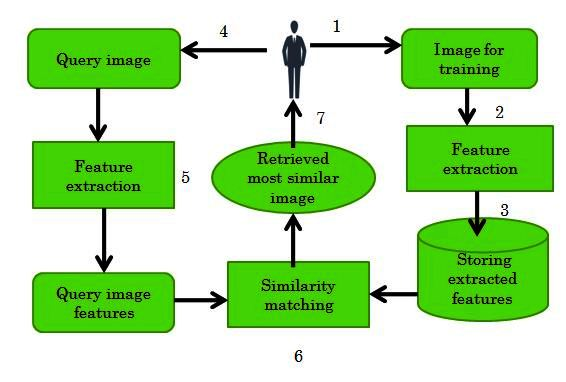
\includegraphics[width=\textwidth]{e.jpg}
           		\caption[Architecture of existing system]{Architecture of existing system (CBIR)}
             		\label{Invite friends}
		\end{center}
	\end{minipage}
\end{figure}

\vspace{1pc}
\subsection[CBIR Algorithm:]{CBIR Algorithm:}
\begin{algorithm}
	\caption{CBIR Algorithm to  retrieve most similar image for query image}
	Input: Query image\\
	Output:Most similar images to  the input image\\
	\begin{algorithmic}
		\State Give input image
		\State Extract the feature vector for the input image 
		\State Calculate the weighted features vectors for the input image
		\State Calculate the distance between the input image and the centroid of each K-mean  cluster  and find  the smallest distance
		\State Calculate the distance between the input image and the images in the cluster that has the smallest distance with the input image
		\State Retrieve   most similar images to the input image
	\end{algorithmic}
\end{algorithm}
\clearpage
\end{comment}

\subsection[Wristbands for the identification and tracking of patients]{Wristbands for the identification and tracking of patients} 
It is possible to associate a passive RFId tag to a patient by means of a wristband. Patient automatic identification using non-transferable wristbands enables a number of benefits: 


\begin{enumerate}
	\item it helps improving the efficiency of the system, it provides quick access to clinical and personal data of a patient that are stored within the information system (for read/write and transfer operations), including an improvement of communications; 
	\item it increases patient safety, it reduces errors (for example, the problems caused by the use of drugs or surgery on the wrong patient, the risk of incorrect medical treatments or interventions onto the wrong parts of the patient’s body); 
	\item reading a tag is faster than reading a bar code and, unlike the reading of bar codes, it can be carried through and around the human body, through clothes, through the blankets of the bed and through non-metallic materials, without disturbing the patient;
	\item tags provide greater security on bar codes, which are easier to copy and duplicate; 
	\item there are printers and programmers to print and program the wristbands.
\end{enumerate}

\subsection[Localization of equipment, patients and medical staff]{Localization of equipment, patients and medical staff} 
It is possible to realize an approximate tracking system, placing the reader at the entrance of the hospital premises. The tags can be placed on patients, in the identification badges of workers (medical staff and other workers), on various equipment (including medical devices). 

\begin{figure}[h!]
	\centering
	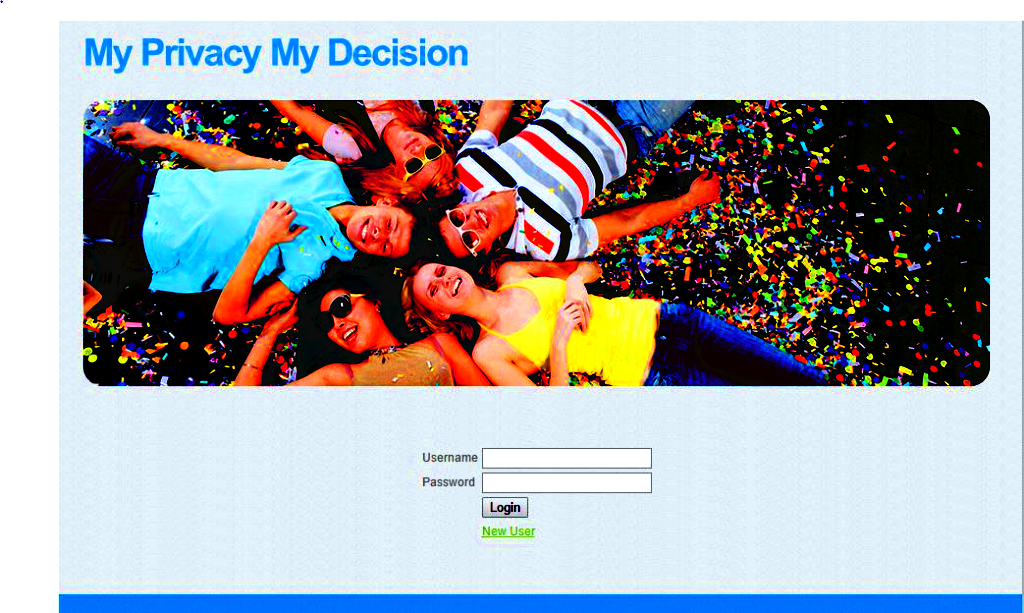
\includegraphics[scale=1]{1.png}
	\caption[Possible situation in an operating room where tags are used]{Possible situation in an operating room where tags are used}
\end{figure}

The following are possible features that integrate and extend what has already been shown (figure 1): 

\begin{enumerate}
	\item tracking of patients and state of the prescribed medical treatment; 
	\item recording of the length of stay of a patient in the emergency room, in wards, in the operating room (including the entire stay in the health facility); 
	\item periodic statistical analysis of data from patients with similar diseases, thanks to the recording in the historical archives of the hospital, in order to improve the management of patients and to verify the achievement of appropriate quality objectives; 
	\item location of medical devices within the premises and their detection in real time; 
	\item emergency management (tracking of patients and workers during emergencies, including any exodus); 
	\item affixing tags to patient records, so as to avoid errors in their compilation or loss or exchange; 
	\item affixing tags to boxes of drugs, to easily locate them; 
	\item tracking of workers (medical staff, nurses and other workers) and patients in health care facilities for the treatment of infectious diseases, in order to identify and pinpoint any necessary treatment in case of breach of the containment of pathogens.  
\end{enumerate}

\subsection[Tracking of surgical instruments in the operating room]{Tracking of surgical instruments in the operating room} 
A typical application of what has been discussed in section IV of this paper may be that of the control of surgical instruments in an operating room: passive tags are placed on the surgical instruments, a reader at their container may signal, after the end of the operation, if an instrument has not been placed back (and also it may indicate which one, thanks to the tag identifier).  

\vspace{1pc}
Also a portable reader can be passed on recently operated patients to ensure that there aren’t instruments left inside their bodies after the operation. There may also be tags to be placed on gauzes and bandages (at predetermined distances), that are certified as safe for such use.  Such a system wouldn’t serve to avoid the adoption of quality procedures for the tracking of surgical instruments and gauzes, but could be used to obtain information (in real time) on the eventual stay of foreign bodies within the patient. 

\subsection[Usage of active devices]{Usage of active devices} 
In the medical practice one can resort to use active devices, for example one can use: 

\begin{enumerate}
	\item active tags for monitoring vital signs/biological parameters (blood pressure, heart rate, blood sugar); 
	\item active tags for monitoring active implantable devices (hearing devices, devices for viewing, devices for periodic release of medicines); 
	\item active tags for monitoring the state of the treatment and the environmental conditions of the place where the patient is.  
\end{enumerate}

\vspace{1pc}
The use of tracking technologies can allow an extension of treatments and cures that can be administered at the patient's house, allowing the reduction of hospitalization costs. This can be especially useful in the case of chronic patients, people with reduced mobility, elderly, infants. It is sufficient that readers be positioned at the houses and networked with the information system of the health facility. 

\section[USAGE FOR THE IMPROVEMENT OF THE ACCURACY OF EXCAVATIONS IN THE SUBSOIL]{\fontsize{14}{12}\selectfont USAGE FOR THE IMPROVEMENT OF THE ACCURACY OF EXCAVATIONS IN THE SUBSOIL}
During digging operations in the subsoil, carried out for the maintenance of distribution networks (e.g.: electrical network, telephone network, water mains, gas mains, sewage network, public lighting network), it may be difficult to recognize the network on which one has to intervene or, once identified the network, to locate the exact spot on which one should intervene. This happens because of delays in the communication of updated maps or because of inaccuracies on such maps, regarding the listing of distances and the georeferenced.  

\vspace{1pc}
Often the consequences of this are delays in performing operations, discomfort for road users that live in cities under which the networks develop in the subsoil, as well as errors and accidents (damages to other networks in the vicinity of those that are subject to intervention), with repercussions in the event of major accidents, even on the safety of workers in charge of the excavation. 

\vspace{1pc}
By equipping the various networks with tags, with a discontinuous distribution (tags located along the track, in singular points, in equipment, in piping or accessories) or with a continuous distribution (tags placed in sequence and briefly spaced), it is possible, through interrogation with portable readers, standing on the surface, to obtain detailed information of the networks in the subsurface.  

\vspace{1pc}
Tags can be placed along the networks in the construction phase or during the subsequent maintenance. Systems whose operating frequency differs depending on the type of network are already in use. This methodology of detection can arrive deep in the soil up to 2.5 m, by using passive tags, which do not require power, in robust casings that are able to resist to chemicals, to high temperatures and pressures which can occur in the subsoil.  

\vspace{1pc}
The information that can be obtained range from the type of network to the materials with which the piping is made, from the three-dimensional position (referenced with GPS information) of piping and accessories (boxes, derivations), to the history of maintenance operations which the particular section of the network has undergone, and to the composition, structure and consistency of the soil. 

\begin{comment}
%%%%%%%%%%%%%%%%%%%%%%%%
%-----------------------------------------------------------------------------------------------
%%%%%%%%%%%%%%%%%%%%%%%%%%%%%[ PRROBLEM DEFINITION ]%%%%%%%%%%%%%%%%%%%%%%%%%%
\addtocontents{toc}{\cftpagenumberson{chapter}}
\chapter[PROBLEM DEFINITION]{\fontsize{16}{12}\selectfont PROBLEM DEFINITION}
\noindent
In a typical CBIR system, low- level visual image features that is colour, texture, and shape are automatically extracted for image descriptions and indexing purposes. To search for desirable images, a user presents an image as an example of similarity, and the system returns a set of similar images based on the extracted features  The main issue with CBIR system is the time of image retrieval in almost all CBIR systems depends in a large degree on the number of images in the database.

%% % \nointent
  \vspace*{1pc} 
Two main issues with CBIR systems are efficiency and accuracy. Hence, an effective CBIR system needs to have an efficient search mechanism and also accurate set of features. Out of all the mechanisms used in CBIR, k-means clustering is found to have better efficiency and accuracy. 
"Content-based" means that the search will analyze the actual contents of the image rather than the metadata such as keywords, tags, and/or descriptions associated with the image. The term 'content' refer to colours, shapes, textures, or any other information that can be derived from the image itself.
 CBIR is desirable because most web based image search engines rely purely on metadata and this produces a lot of garbage in the results. Also having humans manually enter keywords for images in a large database can be inefficient, expensive and may not capture every keyword that describes the image.
 
 %% \nointent
  \vspace*{1pc}
   Thus system that can filter images based on their content would provide better indexing and return more accurate results. Again the performance of the CBIR system is improved by using K-Means clustering technique .If we are using CBIR to train individual’s images and for face recognition in our proposed system. To get enough training sample is actually little difficult task, so FR engine may be unsuccessful to identify the faces of each individual in a group photo.FR engine could be trained to recognize social friends (people in social circle) but to get enough training sample is a difficult task.To get efficient result CBIR demands more training samples (photos of each specific person), but online photo resources are often insufficient, also with varying poses and facial expressions CBIR system may fail to recognize the faces of each individual in a group photo. More demanding privacy setting may limit the number of the photos publicly available to train the FR system..Another major issue we are facing is large number of users are absent for us to carry out the network-wide evaluation. We simulate a real-life social network with the small-world network.
 \clearpage
%%%%%%%%%%%%%%%%%%%%%%%[ MODIFICATION ]%%%%%%%%%%%%%%%%%%%%%%%%%%%%%%
\addtocontents{toc}{\cftpagenumberson{chapter}}
\chapter[METHODOLOGY]{\fontsize{16}{12}\selectfont METHODOLOGY}
\noindent
The proposed system is used to reduce the privacy leakage issues while uploading a photo through OSNs.CBIR algorithm is used for face recognition in the proposed system.CBIR algorithm is one of the most popular algorithm used for image retrieval.CBIR system  defines the similarity between contents of two images based on global feature(i.e. features extracted from the whole image).The proposed system  using Haar cascade classifier for face detection,it crops all the face regions from the images ,so need not find the similarity based on global feature.

 %% \nointent
  \vspace*{1pc}
  To curb the privacy leakage, we proposed to enable individuals potentially in a photo to give the permissions before posting a co-photo. We designed a privacy preserving Content based image retrieval FR system to identify individuals in a co-photo.Face detection is an important part in the proposed system because in the proposed system each co-photo owners are participating in the decision making of photo uploading through social networks.\vspace{1 pc} The proposed system is featured with low computation cost and confidentiality of the training set.  The proposed system added time limit for notification acceptance, and SMS notification to inform the co-photo owner about the time limit for notification. We expect that our proposed scheme be  very useful in protecting users’ privacy in photo/image sharing over online social networks.
\section[Proposed System Architecture]{\fontsize{14}{12}\selectfont PROPOSED SYSTEM ARCHITECTURE}
%\subsection[Admin]{Admin}
\begin{figure}[H]
\begin{minipage}{1\linewidth}
\centering
\begin{center}
 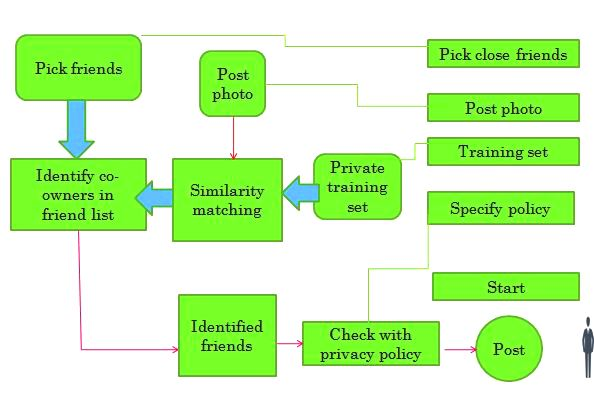
\includegraphics[width=\textwidth]{p.jpg}
           % \text{\scriptsize(ISO 9001:2008 Certified)}
            \caption[Proposed System Architecture]{Proposed system Architecture}
             \label{Invite friends}
\end{center}
\end{minipage}
\end{figure}
%\clearing
\subsection[Start]{Start}
%\noindent
%4.1.1Start
User can register to Online Social Network by entering the details like name, DOB, gender, Email, mobile number, user name, password etc. Once registered successfully user can login to his/her account. User or admin can login to this system if they have a valid user id and password. Admin can login with a valid password, once login admin can view the user details. Main function of admin is to train the user image
\subsection[Specify Policy]{Specify policy}
%\noindent
%4.1.2 Specify policy
We assume that each user u has a privacy policy$Pu(i)$ and a exposure policy $Eu(i)$ for a specific photo$ i$. The privacy policy $Pu(i)$ indicates the set of users who can access photo$ i $
.In our project we set two options ,one is view public and net is view my friends.If a user is selecting public option ,once photo is uploaded  that photo will be shown publically ,if he/ she is setting only my friends option then once the photo is  uploaded ,it  will be available in the time line of his/her friends home page.Exposure policy $Eu(i)$ indicates the set of users who can access$ i$ when user $u$ is involved.In our project we limited this within the close friend list. According to our scheme, this friend list should be intersection of owner’s privacy policy and co-photo owners’ exposure policies. At present, when the push button “Post Photo” is pressed, co-owners of$ i$ are identified, and then notifications along with $i$ are sending to the co-owners  within the close friend list to request permissions. If they all agree to post$ i$, $i$ will be shared on the owner’s page like a normal photo. In this sense, users could specify their privacy policy but their exposure policies are depends the set of users who can access $i$ when user $u$ is involved.
\subsection[Training]{Training}
%\noindent
%4.1.3 Training
A log in/out button could be used for log in/out with our social network site. After login , user can train their individual images , we need an efficient content based image retrieval facial recognition (FR) system that can used to train users images. We are using Haar cascade classifier for face detection and CBIR algorithm to train individual’s images and for face recognition.  FR engine could be trained to recognize social friends (people in social circle) but to get enough training sample is a difficult task.
 
 %% \nointent
  \vspace*{1pc}
FR engine with advanced recognition ratio demands more training samples. In the training phase, both decomposition and feature extraction takes place. Haar Wavelet Transform is used for calculating the feature vectors, weighted feature vector represented as weight function w(). Then k-means clustering algorithm is used for clustering the images based on their feature vectors , considering the minimum Euclidean distance. The basic idea is to transfer an image into matrix in which each element of the matrix represents a pixel in the image. A Haar Wavelet transform decomposes an image into two components: average and difference.Each color in the image can be represented by considering the pixels as a point in space and from this matrices for each Red, Green and Blue components of RGB are constructed. This is then decomposed into four sub matrices through row and column transformations[Appendix-A].
 % \thispagestyle{empty
%\begin{enumerate}[label=(\roman*)]
\begin{description}
\item[(i)]  The formula for calculating average and difference at level 1 is given by
%The formula for calculating average at level 1 is given by}
%\end{enumerate}
The formula for calculating average is shown in equation(4.1):
\begin{equation}\label{}
avg = \frac{f_n+f_{n+1}}{\sqrt{2}}, \text{where n} = 1,2,3,.....\frac{n}{2}
\end{equation}

And difference at the same level is shown in equation(4.2):
\begin{equation}\label{}
diff = \frac{f_n-f_{n+1}}{\sqrt{2}},\text{where n}=1,2,3,.....\frac{n}{2} 
\end{equation}
%\thispagestyle{empty}
%\begin{enumerate}(ii)

\item[(ii)]To calculate the Haar transform of an array of n samples: 
%\end{enumerate}
       \begin{enumerate}
 \item Find the average of each pair of samples. (n/2 averages) 
 \item  Find the difference between each average and the samples it was calculated from. (n/2 differences) 
 \item  Fill the first half of the array with averages 
 \item  Fill the second half of the array with differences. 
 \item Repeat the process on the first half of the array. While doing this the array size should be power of two.
\end{enumerate}
\end{description} 
This steps are repeated for both row and column. Once the process is completed, the matrix gets decomposed into four sub-matrices each of dimension (number of rows/2) x (number of
columns/2) and is called A, H, V and D respectively. A (approximation area) contains
information about the analyzed image’s global properties, H (horizontal area) contains
information about vertical lines hidden in the image, V (vertical area) contains information about the horizontal lines hidden in the image and D (diagonal area) contains information about the diagonal details hidden in the image.
%\begin{enumerate}(ii)
\begin{description}
\item[(iii)] The advantages of Haar Wavelet transform: 
%\end{enumerate}
\begin{enumerate}
\item  Best performance in terms of computation time 
\item Computation speed is high 
\item Simplicity 
 \item HWT is efficient compression method
\end{enumerate}
\end{description} 
Once decomposition is done, then feature vectors can be constructed using mean and standard
deviation of energy distribution ( $F$-norm) of each sub-band at each level. The equation for calculating $F$-norm  is shown in equation(4.3)
Given a square matrix$A$ and $A_i$ is  a sub matrix from it, then $F$- norm given by,
\begin{equation}
|A_i|_{F} =\left[ \sum\limits_{k=1}^i \sum\limits_{k=1}^i|a_{kl}|{^2} \right]^{\frac{1}{2}}
\end{equation}
The equation for calculating mean($\mu$)is shown in equation(4.4)
 \begin{equation}
%\text{Mean($\mu$)}=\frac{\sum \text{F-norm}}{\text{no of columns of F-norm}}}
\end{equation}
The equation for calculating standard deviation($\sigma$)is shown in equation(4.5)
 \begin{equation}
\text{StanderdDeviation($\sigma$)} = \sqrt{\frac{\sum \left(\text{F-norm}- mean\right)^2}{\text{no of columns of F-norm}}}
\end{equation}
The equation for calculating variance($\sigma^{2}$)is shown in equation(4.6)
 \begin{equation}
\text{Variance($\sigma^{2}$)} = \Bigg(\sqrt{\frac{\sum \left(\text{F-norm}- mean\right)^2}{\text{no of columns of F-norm}}}\Bigg)^{2}
\end{equation}

 %%%%%%%%%%%%%%5
 \begin{description} 
 \item[(iv)]K Mean Algorithm
 %\end{description}  
The basic step of k-means clustering is simple. In the beginning, determine number of cluster K and assume the centroid or center of these clusters. We can take any random objects as the initial centroids or the first K objects can also serve as the initial centroids. Then the K means algorithm will do the three steps below until convergence[12].
    % \begin{enumerate}
    % \item aaaaaaaaaaaaaaaaaaaaaaaaaaaaa
     %\item bbbbbbbbbbbbbbbbbbbbbbbbbbbb
     %\item cccccccccccccccccccccccccccccc
    % \end{enumerate}
     \end{description}     
      \begin{algorithm}
\caption{K-Mean  Algorithm }
   Input: Number of cluster k,N objects\\
   Output:A set of K clusters\\
\begin{algorithmic}[1]
\State Arbitrarily choose k objects as the initial cluster centers.
\State (Re)Assign each objects to the cluster to which the object is the most similar based on the mean value of objects in the cluster.  
\State Update the cluster means,i.e, calculate the mean value of the objects for each cluster.
\State Repeat steps 2 and 3 until no changes.
\end{algorithmic}
\end{algorithm}
%\end{enumerate}
 %\end{roman} 
%%%%%%%%%%%%%%%%%
 \subsection[Pick Friends]{Pick friends}
 \noindent
 %4.1.4 Pick friend
User can search through this social networking site to get friends ,there is an invite friend option to find friends, user needs to set “close friends” among their Social Network friends either by sending friend request or accepting others friend request. When a person try to upload a group photo, FR system identify all co-photo owners from this close friends group.
\subsection[Photo Uploading]{Photo uploading}
\noindent 
%4.1.5 Photo Uploading
Once  user is logging in to his/her account, he/she can use the photo posting feature of OSN.
In this phase, when an image is uploaded,all the faces in the images is detected by open CV  face detection  using Haar Cascades. Once each faces are croped from the given image then its feature vectors are computed using the same procedure which we have done in training image. This vector is compared to the vectors of images in the training set using Euclidean distance.

%% % \nointent
  \vspace*{1pc}
The classification of the most similar images would be returned as the class of the newly uploaded image, similarity function represented sim() , then checking  the recognized faces are in  the friend list of uploader. When posting a group photos on online social network an automatic acceptance notification is sending to the co photo owners in the close friend circle  informing their presence in that group photo, so each co-photo owners are getting the chance to view the photo where they are in before the up loader post the photo and any one of them press reject button nobody can upload that photo, if all are pressing acceptance button, then only the photo will be posted. More over we set a time limit for the notification acceptance(5 days),  if the time limit is exceeded the photo will be uploaded automatically otherwise if co-photo owners are not login to this system for long then nobody can use photo sharing feature of OSNs.Sometimes the co-photo owners are unable to login to this account within the time limit but photo will be uploaded after the time limit,it will become another privacy issues. To avoid this issue we can add SMS notification  to inform each co-photo owners about the photo uploading and time limit, so it is useful them to login to the system and either accept or reject the notification.

% % \nointent
  \vspace*{1pc}
Proposed system is used to prevent possible privacy leakage of a photo, this mechanism is enabled each person in a photograph be aware of the posting the photograph and actively participate in the decision making on the photograph posting.
\clearpage
\subsection[Flow Diagram]{Flow Diagram}
%%%%%%%%%%%%%%%%%%%%%%%%%%%%%%%% 
% \begin{figure}[H]
% \centering
%  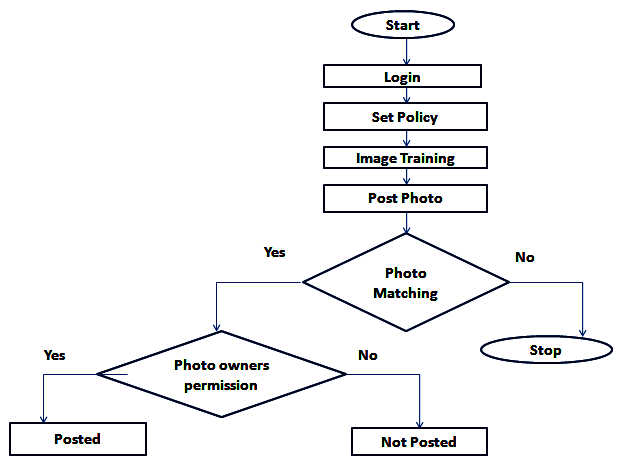
\includegraphics[scale=1]{flowgraph.png}
 % \caption[Proposed System Flow Graph]{Proposed system flow graph}
 % \label{pf}
%\end{figure}
%%%%%%%%%%%%%%%%%%%%%%%555
\vspace{2cm}
\begin{figure}[H]
\begin{minipage}[c]{1\linewidth}
\begin{center}
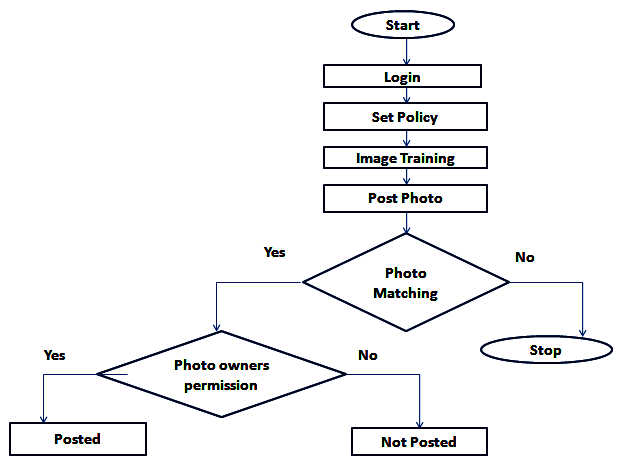
\includegraphics[width=\textwidth]{flowgraph.png}
           % \text{\scriptsize(ISO 9001:2008 Certified)}
           \caption[Proposed System Flow Graph]{ Proposed system flow graph}
             \label{Posted }
\end{center}
  \end{minipage}            
\end{figure}
%%%%%%%%%%%%%%%%%%%%%%%%%%%%%%%%%%
The flow graph shown in figure 4.2 shows  the entire flow of proposed system clearly.Start with user login,Image training, policy setting,photo uploadind, notification sending and Finally collect the decision from each co-photo owners, if all are agreed to upload the  image,then  photo posting is granted else not granted.
\clearpage
\section[Proposed Algorithm]{\fontsize{14}{12}\selectfont PROPOSED ALGORITHM}
\subsection[CBIR Algorithm:]{CBIR Algorithm:}
\begin{algorithm}

\caption{CBIR Algorithm to  retrieve most similar image for query image}
   Input: Query image\\
   Output:Most similar image to  the input image\\
\begin{algorithmic}[1]
\State Give input image which contain one or more faces
\State Detecting all faces in the image.
\State Extract the feature vector for the input image 
\State Calculate the weighted features vectors for the input image
\State Calculate the distance between the input image and the centroid            of each K-mean  cluster  and find  the smallest distance

\State Calculate the distance between the input image and the images
            in the cluster that has the smallest distance with
             the    input image

\State Retrieve   most similar image to the input image  and Send acceptance 
            notification to co -photo owners within the close circle.


\end{algorithmic}
\end{algorithm}

% % \nointent
  \vspace*{1pc}
CBIR algorithm is used for face recognition in the proposed system.CBIR algorithm is one of the most popular algorithm used for image retrieval.The proposed system  using Haar cascade classifier for face detection,it crops all the face regions from the images ,so need not find the similarity based on global feature.in the proposed algorithm we are  giving face images  which is croped using  Haar cascade classifier to the CBIR system , then find  the feature vector for each and calculate  Euclidean distance to get most matching image ,the image which is already trained and saved in cluster files.Our proposed scheme be  very useful in protecting users’ privacy in photo/image sharing over OSNs.
\clearpage

\section[System Designs]{\fontsize{14}{12}\selectfont SYSTEM DESIGNS}
%4.2 SYSTEM DESIGNS	
This section explains various designs used for the project,they are use case diagrams of admin and user, admin's and user's data flow diagrams.These diagrams help to understand the entire operations of the system.This section also explains various tables used for the project.The relational database management system MySql server is used for this purpose.

\subsection[Use Case Diagrams]{Use Case Diagrams}
In this Project there are mainly two parts user and admin. Use case diagram  of admin shown in figure 4.3.Admin can login with a valid password, once login admin can view the user detals like username, profile picture, email id, mobile phone number, moreover admin can do the performance analysis. Performance analysis is done based on time taken (mille seconds)to train an  image, face detection and face recognition. It can be  displayed using a bar chart.  main function of admin is to train the user image and saving values corresponding to each image in a cluster file for later search process
\begin{figure}[H]
 \centering
  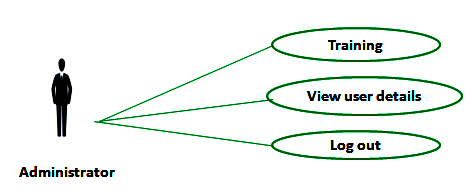
\includegraphics[scale=0.8]{au.png}
  \caption[Admin:Use Case Diagram]{Admin:Use case diagram}
  \label{pf}
\end{figure}
%%%%%%%%%%%%%%%5
This project is based on social networking platform, so most of the operations are done by user. Use case diagram  of user is  shown in figure 4.4.In this system an  individual can create an account using “new registration option”, then user can login with a valid username and password, user can select his/ her image for taining purpose, once image selected admin will do the training process. User can choose friends by using invite friend option. Policy setting is an important part in this project, if user is selecting the notification checkbox then only he/she will get the notification whenever somebody is trying to upload his / her photo. Photo uploading is the main part done by user, here face detection and recognition is take part.
\begin{figure}[H]
 \centering
  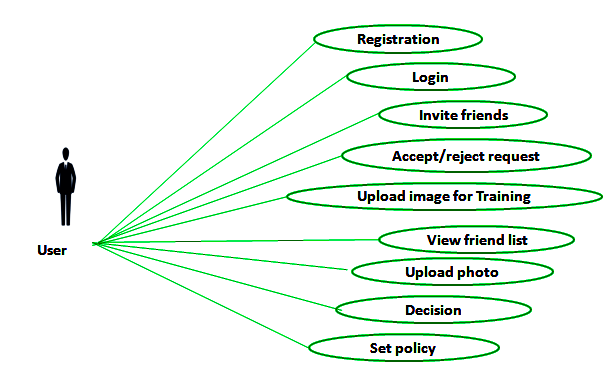
\includegraphics[scale=0.8]{uu.png}
  \caption[User:Use Case Diagram]{User:Use case diagram}
  \label{pf}
\end{figure}
\subsection[Data Flow Diagrams]{Data flow diagrams}
\noindent
\justifying
This section discuss the design of the proposed system.Figure 4.5 gives the descriptions of the notations used in the flow diagram.Rectangle represents an entity, a source of data or destination for data.Processes are the tasks that are performed by the system.Label the arrows with the name of the data that moves through it.Data stores are repositories of data in the system.
%%%%%%%%%%%%%%%%%%%%%%%%%%%%%%%
 \begin{figure}[H]
 \centering
  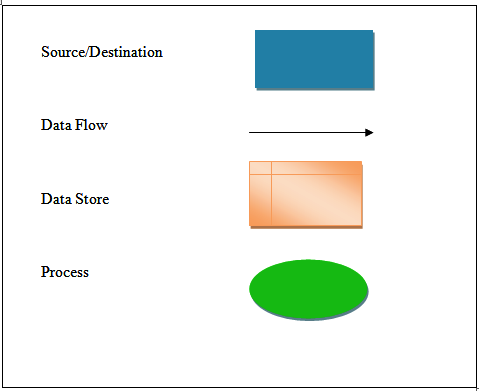
\includegraphics[scale=1]{ndfd0.png}
  \caption[Data Flow Diagram Notations]{Data flow diagram notations}
  \label{pf}
\end{figure}
%%%%%%%%%%%%%%%%%%%%%%%%55

\begin{figure}[H]
\begin{minipage}[c]{1\linewidth}
\begin{center}
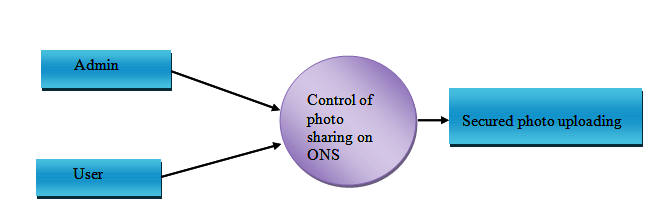
\includegraphics[width=\textwidth]{ndfd1.png}
           % \text{\scriptsize(ISO 9001:2008 Certified)}
         \caption[Context Level DFD]{ Context level DFD}
             \label{Posted photo on time line of Social Networking site}
\end{center}
  \end{minipage}            
\end{figure}
%%%%%%%%%%%%%%%%%%%
\begin{figure}[H]
\begin{minipage}[c]{1\linewidth}
\begin{center}
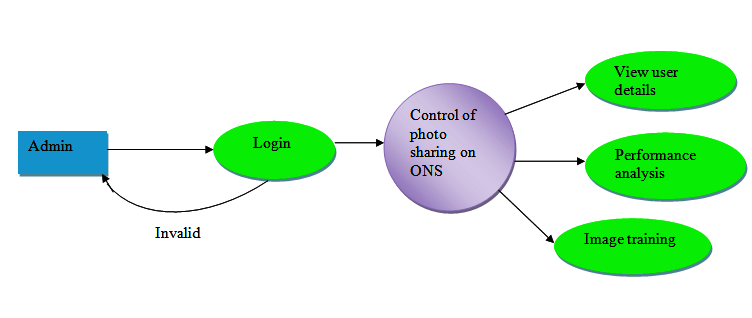
\includegraphics[width=\textwidth]{ndfd2.png}
           % \text{\scriptsize(ISO 9001:2008 Certified)}
        \caption[Admin: level 0 DFD]{ Admin: Level 0 DFD}
             \label{Posted photo on time line of Social Networking site}
\end{center}
  \end{minipage}            
\end{figure}
%%%%%%%%%%%%%%%%%%%%%%%%%%%
\begin{figure}[H]
\begin{minipage}[c]{1\linewidth}
\begin{center}
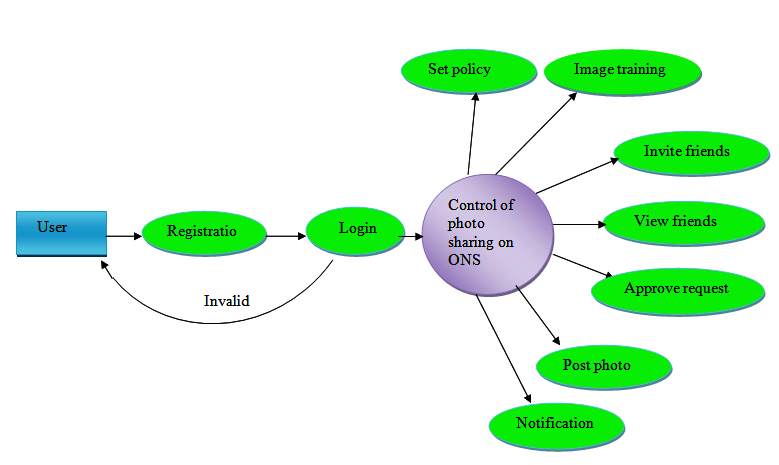
\includegraphics[width=\textwidth]{nndfd2.png}
           % \text{\scriptsize(ISO 9001:2008 Certified)}
           \caption[User: level 0 DFD]{ User: Level 0 DFD}
             \label{Posted photo on time line of Social Networking site}
\end{center}
  \end{minipage}            
\end{figure}
%%%%%%%%%%%%%%%%%%%%%%
\begin{figure}[H]
\begin{minipage}[c]{1\linewidth}
\begin{center}
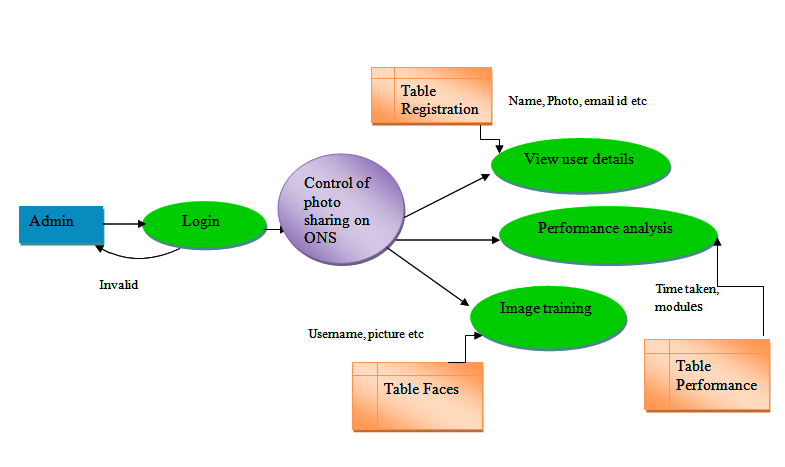
\includegraphics[width=\textwidth]{ndfd4.png}
           % \text{\scriptsize(ISO 9001:2008 Certified)}
           \caption[Admin: Level 1 DFD]{ Admin: Level 1 DFD}
             \label{Posted photo on time line of Social Networking site}
\end{center}
  \end{minipage}            
\end{figure}
%%%%%%%%%%%%%%%
\begin{figure}[H]
\begin{minipage}[c]{1\linewidth}
\begin{center}
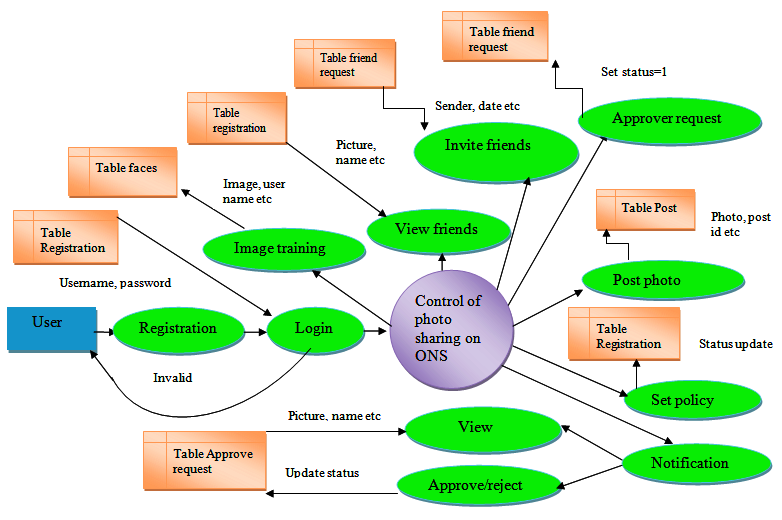
\includegraphics[width=\textwidth]{nndfd5.png}
           % \text{\scriptsize(ISO 9001:2008 Certified)}
            \caption[User: Level 1 DFD]{ User: Level 1 DFD}
             \label{Posted photo on time line of Social Networking site}
\end{center}
  \end{minipage}            
\end{figure}
\clearpage
%%%%%%%%%%%%%%%%

%%%%%%%%%%%%%%%%%%%%%%%%%%
%\subsection[TB]{Table designs}
\subsection{Table design}
The project require a database for storing details of admin and users  and their operations.This section also explains various tables used for the project.The relational database management system MySql server is used for this purpose.The databse is constantly updated and maintained.

% % \nointent
  \vspace*{1pc}
The database table "approve request" shown in figure 4.11 is used  when a user is uploading a photo using post photo option a post id will be generated , photo uploader name will be added to  the column” From user “ and all the recognized persons who need to get the notifications will be added to the column “ To user”.Initially status will be zero ,any one is accepting the notification then  corresponding status value will be changed to one and any one is  rejecting the notification  then corresponding status will be changed to two.
\begin{figure}[H]
\begin{minipage}{1\linewidth}
\centering
%\begin{center}
 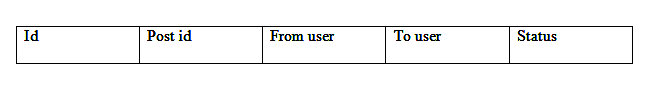
\includegraphics[width=\textwidth]{tb1.png}
           % \text{\scriptsize(ISO 9001:2008 Certified)}
            \caption[Approve Request Table]{Approve request table}
             \label{art}
%\end{center}
\end{minipage}
\end{figure}
% \nointent
\justifying
The database table image training shown in figure 4.12 is used to add details while a user upload his/her photos for training purpose. Initially   values in status column are  zero for all registered users ,once training   is done successfully selected photo for training will be added to the table and status will be updated to the value one.
\begin{figure}[H]   
\begin{minipage}{1\linewidth}
\centering
%\begin{center}
 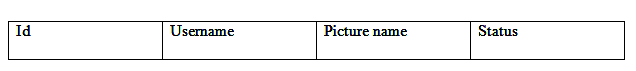
\includegraphics[width=\textwidth]{tb2.png}
           % \text{\scrize(ISO 9001:2008 Certified)}
            \caption[Image Training Table]{Image training table}
             \label{itt}
%\end{center}
\end{minipage}
\end{figure}
% \nointent
\justifying
The database table" friend request" is shown in figure 4.13 is used when a user is sending a friend request to anyone in this project, then the sender’s and receiver’s name will be added to the friend request table .  Initially  values in the status column will be zero and if the receiver is accepting the friend request, status will be changed to the value one.
\begin{figure}[H]
\begin{minipage}{1\linewidth}
\centering
%\begin{center}
 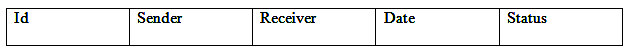
\includegraphics[width=\textwidth]{tb3.png}
           % \text{\scriptsize(ISO 9001:2008 Certified)}
            \caption[Friend Request Table]{Friend request table}
             \label{frt}
%\end{center}
\end{minipage}
\end{figure}
% \nointent
\justifying
The data base table "post" shown in figure 4.14 is used when an user  is posting  a photo, then username , photo used to upload and date of attempt will be added to the table .Initially status will be zero and once the photo is posted, then status will be changed to one.
\begin{figure}[H]
\begin{minipage}{1\linewidth}
\centering
%\begin{center}
 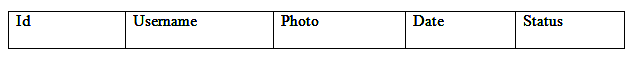
\includegraphics[width=\textwidth]{tbl5.png}
           % \text{\scriptsize(ISO 9001:2008 Certified)}
            \caption[Table Photo Post]{ Table photo post}
             \label{pt}
%\end{center}
\end{minipage}
\end{figure}
% \nointent
\justifying
The data base table "registration" shown in figure 4.15 is used when a person is registering with social networking system,  All user details will be added to this registration table. Here” username” set as primary key. In this table 4.5 privacy policy indicates set of users  who can access the photo , value will be zero if the user selecting” public view” option and the value  will be one if user selecting  “view to my friends” option, if notification policy is selected by user then the corresponding value in the database table will be one otherwise zero.
\begin{figure}[H]
\begin{minipage}{1\linewidth}
\centering
%\begin{center}
 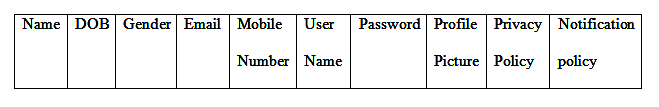
\includegraphics[width=\textwidth]{tbl7.png}
           % \text{\scriptsize(ISO 9001:2008 Certified)}
            \caption[Registration Table]{Registration table}
             \label{rt}
%\end{center}
\end{minipage}
\end{figure}
%%%%%%%%%
% \nointent
\justifying
The data base table "face cutter" shown in figure 4.16 is used when the user is uploading a photo, image will be added to the table ,and no of detected faces in the   photo is added to the” count”  field.
\begin{figure}[H]
\begin{minipage}{1\linewidth}
\centering
%\begin{center}
 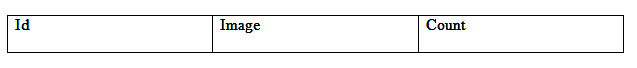
\includegraphics[width=\textwidth]{tbl8.png}
           % \text{\scriptsize(ISO 9001:2008 Certified)}
            \caption[Face Cutter Table]{Face cutter table}
             \label{ft}
%\end{center}
\end{minipage}
\end{figure}

\clearpage
%%%%%%%%%%%%%%%%%%%%%%%[ MODIFICATION ]%%%%%%%%%%%%%%%%%%%%%%%%%%%%%%
%%%%%%%%%%%%%%%%%%%%%%%[ task setup ]%%%%%%%%%%%%%%%%%%%%%%%%%%%%%%
%\addtocontents{toc}{\cftpagenumberson{chapter}}
\chapter[TASK SETUP AND IMPLEMENTATION]{\fontsize{16}{12}\selectfont RESULT AND DISCUSSION}
\section[Modules]{\fontsize{14}{12}\selectfont MODULES}
\subsection[Admin Module]{Admin module}
%\begin{description}
  \begin{description}
\item [(i)]Image training.
%\end{description}
\begin{enumerate}
  \item Face detection.
   \item Image decomposition.
   \item Feature extraction.
   \item Clustering.
\end{enumerate}
\end{description}
\subsection[User Module]{User module}
\begin{description}
\item [(ii)]Photo uploading
\begin{enumerate}
  \item Face Detection.
   \item Face recognition and send notification. 
  \end{enumerate}
\end{description}
\clearpage
\section[System Requirements]{\fontsize{14}{12}\selectfont SYSTEM REQUIREMENTS}
%%%%%%%%%%%%%%%%%%%%%%%%
\begin{table}[H]
\centering
\caption{Software requirement }
\vspace*{.5cm}
\label{routing}
\begin{tabular}{|c|c|}
\hline
\textbf{Parameter} &\textbf{Used for project}        \\
\hline
Operating System  &Windows 8          \\
      
\hline
IDE &NetBeans 7.4            \\
 \hline
Front End &Java7.0 and JSP 2.4          \\
\hline
Back End &MySQL5.0           \\
 \hline
Application Server &Apache Tomcat7.0.41            \\

\hline
\end{tabular}
\end{table}
%%%%%%%%%%%%%%%%%%%%%%%%%%
%%%%%%%%%%%%%%%%%%%%%%%%
\vspace*{1cm}
\vspace*{1cm}
\begin{table}[H]
\centering
\caption{Hardware requirement }
\vspace*{.5cm}
\label{routing}
\begin{tabular}{|c|c|}
\hline
\textbf{Parameter} &\textbf{Used for project}        \\
\hline
Processor &Intel(R)Celeron(r)CPU N2830          \\
      
\hline
Speed&2.16GHz           \\
 \hline
RAM &4GB         \\
Hard Disk &360GB           \\

\hline
\end{tabular}
\end{table}
%%%%%%%%%%%%%%%%%%%%%%%%%%%%%%%



%%%%%%%%%%%%%%%%%%%%%%%[ task setup ]%%%%%%%%%%%%%%%%%%%%%%%%%%%%%%
%\addtocontents{toc}{\cftpagenumberson{chapter}}
\chapter[RESULT AND DISCUSSION]{\fontsize{16}{12}\selectfont RESULT AND DISCUSSION}
\section[Result]{\fontsize{14}{12}\selectfont RESULT}
\noindent
Careless photo posting may reveal privacy of individual in a posted photo. This result enables individuals potentially in a photo to give the permissions before posting a co-photo. I successfully  designed   and tested a privacy-preserving FR system to identify individuals in a co-photo. The proposed system is featured with low computation cost and confidentiality of the training set. Theoretical analysis and experiments were conducted to show effectiveness and efficiency of the work.

% % \nointent
  \vspace*{1pc}
To achive this goal i used CBIR algorithm with K- Mean clustering. The main target of CBIR is to get accurate results with lower computational time.I hope i have done the project with accurate result and lower computational cost.Careless photo posting may reveal privacy of individual in a posted photo. This project result enables individuals potentially in a photo to give the permissions before posting a co-photo.Various web pages of this project is given here.
\clearpage
\subsection[User Registration Page]{User registration page}
To exploit the features of this Online Social Networks every users  need to create an account. User can create a user name and password  User registration page is shown in the figure 6.1.
\vspace{1cm} 
\vspace{1cm}
\vspace{1cm}

 \begin{figure}[H]
\begin{minipage}[c]{1\linewidth}
\begin{center}
 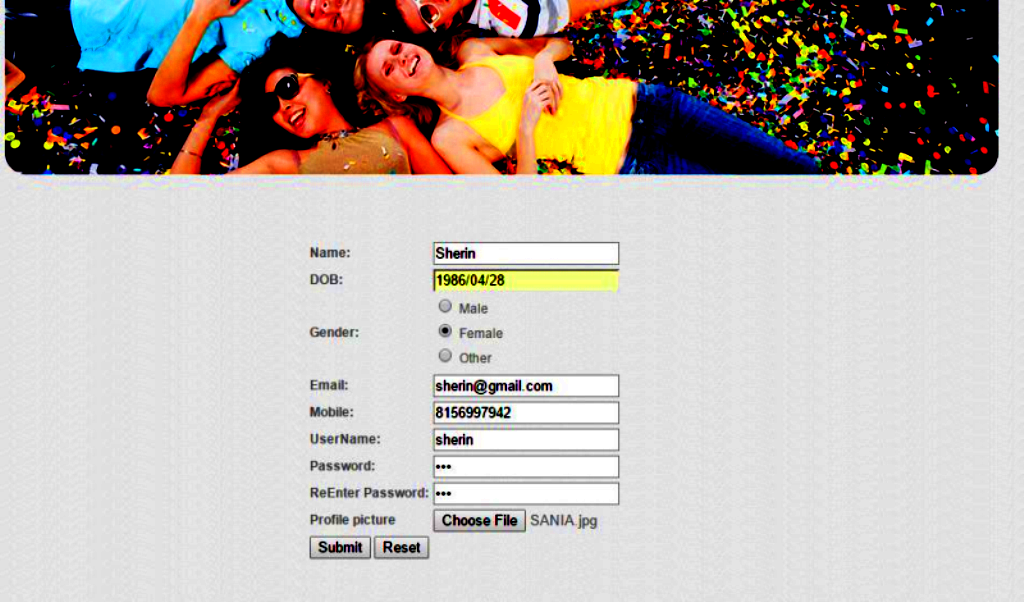
\includegraphics[width=\textwidth]{rej.png}
           % \text{\scriptsize(ISO 9001:2008 Certified)}
        \caption[User Registration Page]{User registration page}
        \label{Login page}
\end{center}
\end{minipage}  
      \end{figure} 
% \clearpage
 \noindent
 \clearpage
 \subsection[Login Page]{Login page}
If registration done successfully user can login to his/her account to explore the features of online social networking.User can login with a valid user name and password.Registration user should enter email id,mobile,number, user name, password etc.Once user login through the page shown in the figure 6.2, then user can use edit profile to edit all the details entered during the  registration time.Administrator can also use the same login page with a valid user name and password.
\vspace{1cm} 
\vspace{1cm}
\vspace{1cm}
\begin{figure}[H]
\begin{minipage}[c]{1\linewidth}
\begin{center}
 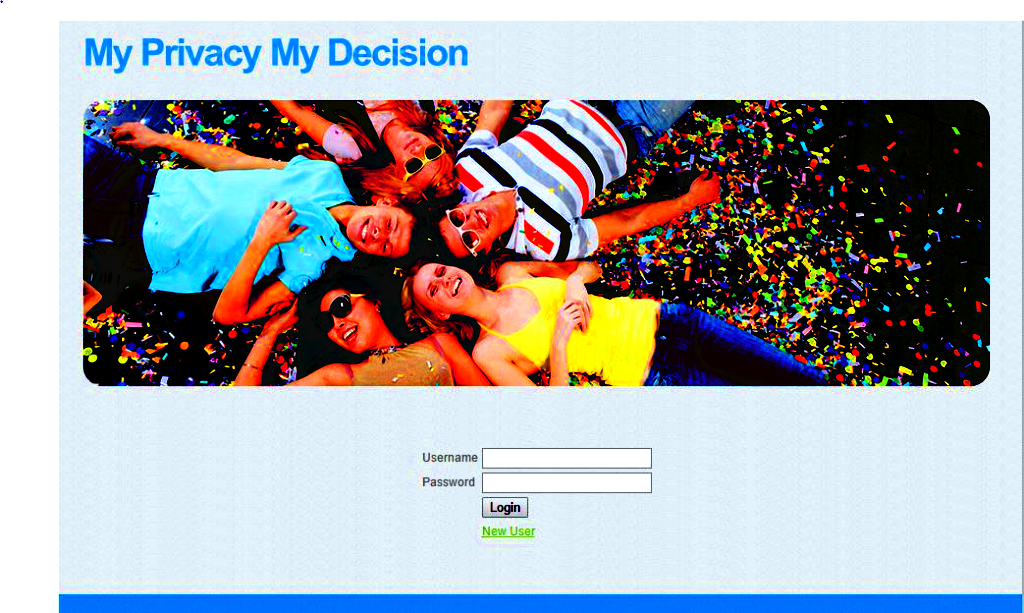
\includegraphics[width=\textwidth]{1.png}
           % \text{\scriptsize(ISO 9001:2008 Certified)}
        \caption[Login Page]{Login page}
        \label{Login page}
\end{center}
\end{minipage}  
      \end{figure} 
% \clearpage
 \noindent
 \clearpage 
 \subsection[Upload Image for Training]{Upload image for training}
Once user login to his /her account then  he/she  can  select an image for training purpose. User should select their own image for training,then only it is possible to get notification while some one else is trying  to upload a photo of them. For better performance user can train the system with more than one images, even using childhood images.User image uploading for training  page is shown in  the figure 6.3.
\vspace{1cm} 
\vspace{1cm}
\vspace{1cm}
\begin{figure}[H]
\begin{minipage}[c]{1\linewidth}
\begin{center}
 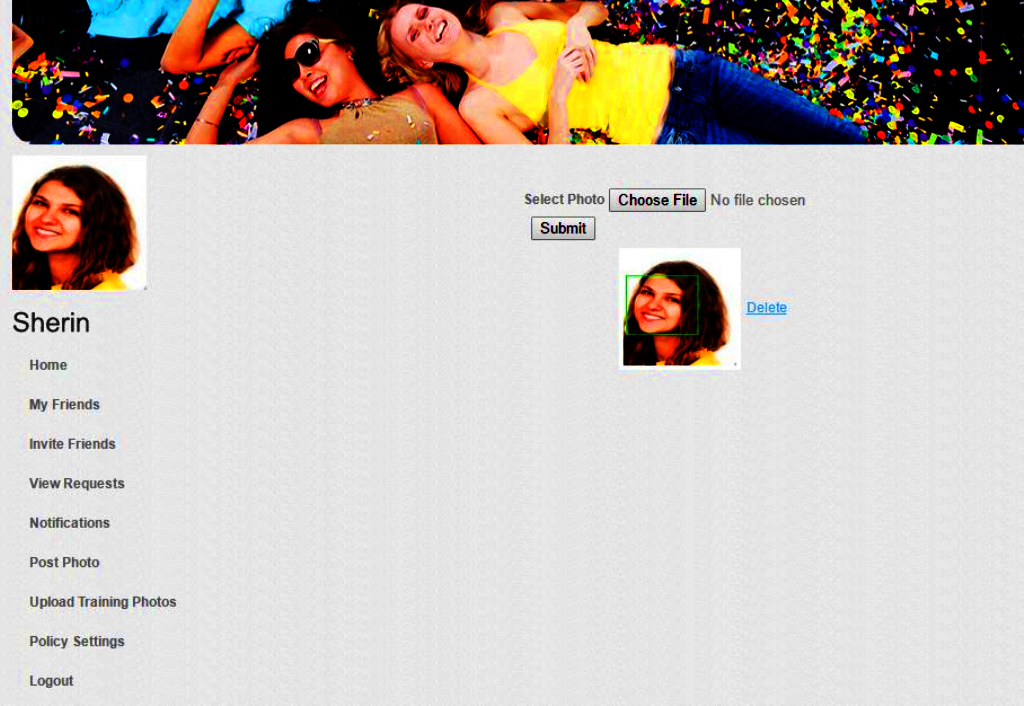
\includegraphics[width=\textwidth]{training2.png}
           % \text{\scriptsize(ISO 9001:2008 Certified)}
      \caption[Upload Image for Training Page]{Upload image for training}
        \label{Upload image for training}
\end{center}

  \end{minipage}  
   
      \end{figure}
      
\clearpage
 \subsection[Image Training Page]{Image training page}
\noindent
Once user select an image and upload it for training, then the notification is going to administrator. Administrator can now train the image.Normally admin is taking six to seven seconds for the training processes.Admin image training  page is shown in the figure 6.4.
\vspace{1cm} 
\vspace{1cm}
\vspace{1cm}
\begin{figure}[H]
\begin{minipage}[c]{1\linewidth}
\begin{center}
 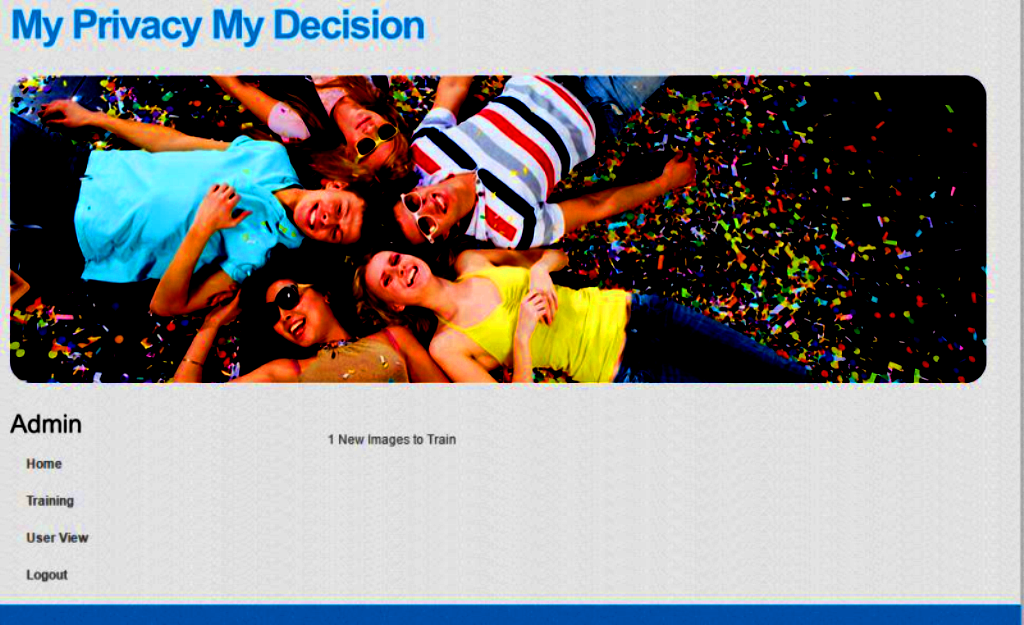
\includegraphics[width=\textwidth]{admintrain.png}
           % \text{\scriptsize(ISO 9001:2008 Certified)}
            \caption[Image Training Page]{Image training page}
             \label{Image training page}
\end{center}
\end{minipage}	
\end{figure}

\clearpage
 \subsection[Invite Friends Page]{Invite friends page}
\noindent
 Once ueser is login with an valid user name and password ,user is able to send a friend request and accept friend request.
To send a friend request user can use invite friend option in the given system, then the name and profile picture with an invite friend option will be displayed and now logged user can invite any one.Invite friends  page is shown in the figure 6.5.
\vspace{1cm} 
\vspace{1cm}
\vspace{1cm}
 
 \begin{figure}[H]
\begin{minipage}[c]{1\linewidth}
\begin{center}
 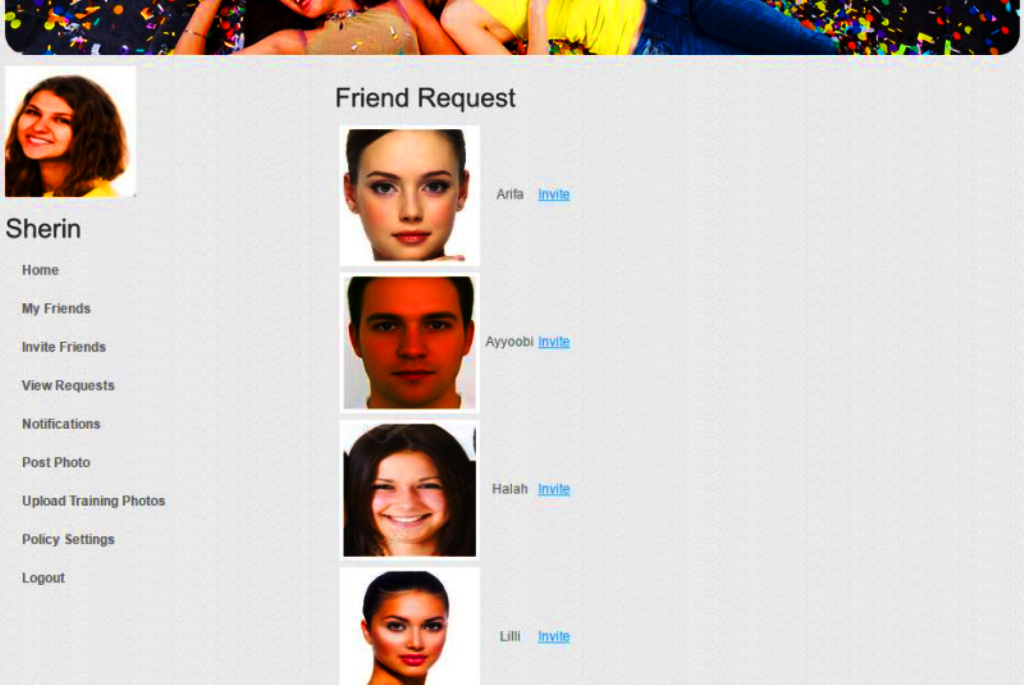
\includegraphics[width=\textwidth]{sherininvitefriends.png}
           % \text{\scriptsize(ISO 9001:2008 Certified)}
            \caption[Invite Friends Page]{Invite friends page.}
             \label{Invite friends}
\end{center}
\end{minipage}
\end{figure}
\clearpage
 \subsection[View Friend Request Page]{View friend request page}
\noindent
 Once user is login with an valid user name and password ,user is able to send a friend request and accept friend request.Logged user can view all  the friend request received by using the option view friend request in this system and user can accept or reject fried request.View friend request page is shown in the figure 6.6.
\vspace{1cm} 
\vspace{1cm}
\vspace{1cm}
 
\begin{figure}[H]
\begin{minipage}[c]{1\linewidth}
\begin{center}
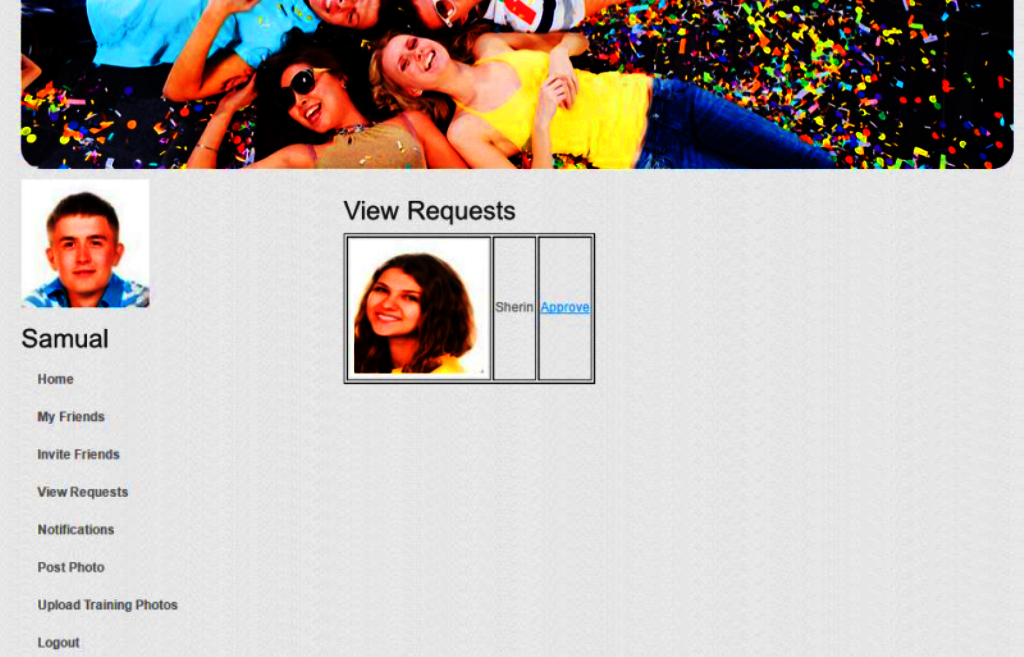
\includegraphics[width=\textwidth]{pendingrequest.png}
           % \text{\scriptsize(ISO 9001:2008 Certified)}
            \caption[View Friend Request Page]{View friend request page}
             \label{View friend request}
\end{center}
\end{minipage}
            
\end{figure}

\clearpage
 \subsection[View Friend List Page]{View friend list page}
 \noindent
 Once user is login with an valid user name and password,user is able to view his/her friend list using the option view friend list in this system.View friend list page is shown in the figure 6.7. 
 \vspace{1cm} 
\vspace{1cm}
\vspace{1cm} 
 
\begin{figure}[H]
\begin{minipage}[c]{1\linewidth}
\begin{center}
 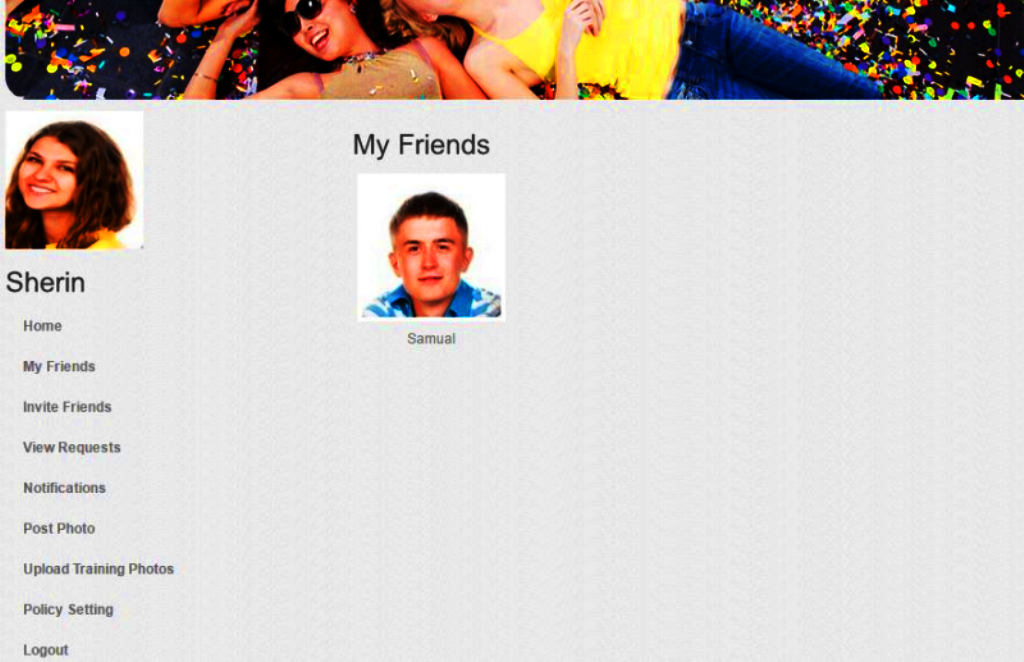
\includegraphics[width=\textwidth]{sherinsfriend.png}
           % \text{\scriptsize(ISO 9001:2008 Certified)}
            \caption[View Friend List Page]{View friend list page}
             \label{Friend list}
\end{center}
 \end{minipage}          
\end{figure}
\clearpage
 \subsection[Post Photo Page]{Post photo page}
\noindent
User can use post photo option in this system to upload any image,to do this user can  browse a   photo from gallery and   upload it by using post photo option.If the image contains human face or faces then Haar cascade  classifier based Face detection  will be activated and cropping all the individual faces from the photo which is being uploading.Post photo page is shown in the figure 6.8. 
 \vspace{1cm} 
\vspace{1cm}
\vspace{1cm}
\begin{figure}[H]
\begin{minipage}[c]{1\linewidth}
\begin{center}
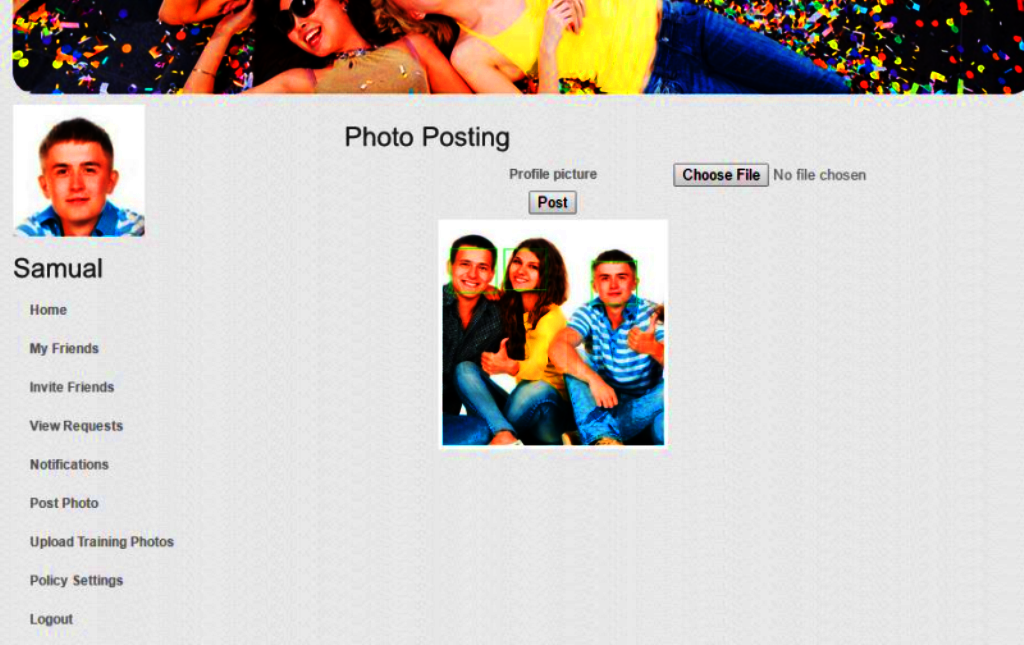
\includegraphics[width=\textwidth]{post.png}
           % \text{\scriptsize(ISO 9001:2008 Certified)}
            \caption[Post Photo Page]{Post photo page}
             \label{Face Detection}
\end{center}
 \end{minipage}           
\end{figure}
\clearpage
 \subsection[Notification Page]{Notification page}
\noindent
When a user try to upload a group photo , all  individual faces will be detected and FR system  cans recognize everyone in the photo. We are using Open CV Haar cascade classifier  for face detection and CBIR algorithm to train individual images and for face recognition. FR system will identify each individual by comparing their face with  trained set of  images,if a match is found,  sending a notification to co photo-owners within close friend circle  informing their presence.Notification page is shown in the figure 6.9. 
 \vspace{1cm} 
\vspace{1cm}
\vspace{1cm}
\begin{figure}[H]
\begin{minipage}[c]{1\linewidth}
\begin{center}
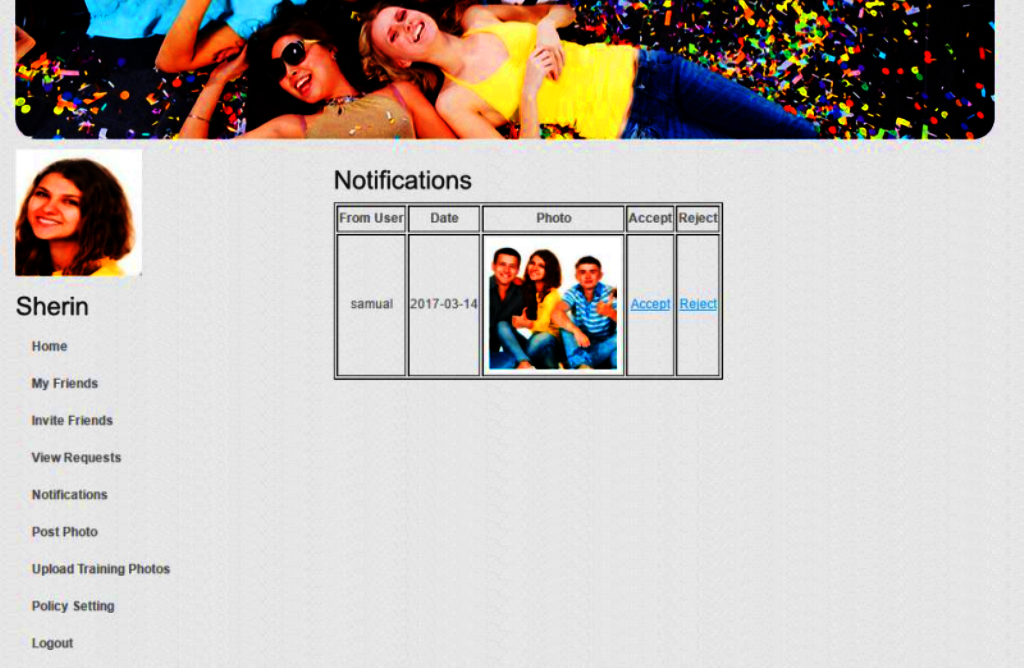
\includegraphics[width=\textwidth]{sherinnew.png}
           % \text{\scriptsize(ISO 9001:2008 Certified)}
            \caption[ Notification Page]{Notification page}
             \label{Notification}
\end{center}
 \end{minipage}             
\end{figure}
\clearpage
 \subsection[ User Time Line Page]{User time line page}
\noindent
If all the notification are accepted by co-photo owners then the  photo will be uploaded  and displayed on the time line page  of  this social networking site.User time line page is shown in the figure 6.10.
\vspace{1cm} 
\vspace{1cm}
\vspace{1cm}
\begin{figure}[H]
\begin{minipage}[c]{1\linewidth}
\begin{center}
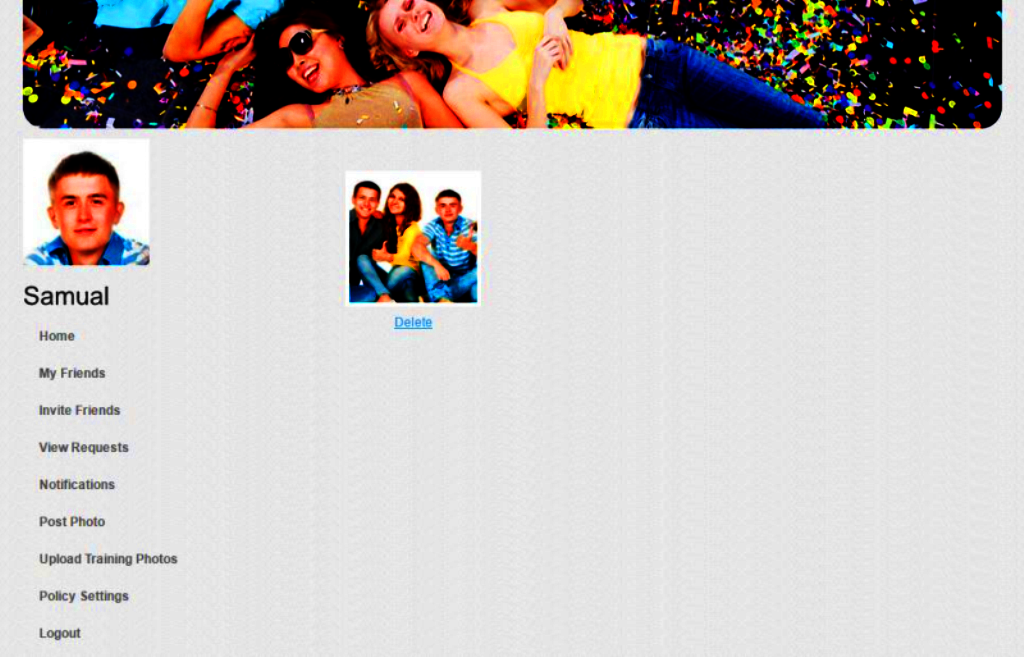
\includegraphics[width=\textwidth]{photoposted.png}
           % \text{\scriptsize(ISO 9001:2008 Certified)}
            \caption[Posted Photo on Time Line of Social Networking Site]{Posted photo on time line of social networking site}
             \label{Posted photo on time line of Social Networking site}
\end{center}
  \end{minipage}            
\end{figure}
\clearpage

\section[DISCUSSION]{\fontsize{14}{12}\selectfont DISCUSSION}
% % \nointent
Control of photo sharing on online social network project work has completed successfully. Various test is conducted during the code generation phase itself. All the errors were rectified at the moment of its discovery. Attention is diverted to individual modules, independently to one another to locate errors.  Registration ,login, photo uploading, privacy policy settings, training individuals images, send and accept friend request ,photo detection, face recognition  and notification acceptance modules tested independently ,this has enabled the detection of errors in coding and logic. To test the efficient working  of  face recognition, we train this system by more than one photos with different  expressions and got successful result.To test the human face detection capability of haar cascade classifier, we tested with various face images, non face images and even with animal faces and got successful result. Finally all these modules are integrated in a master page and tested successfully.

% % \nointent
  \vspace*{1pc}
Careless photo posting may reveal privacy of individual in a posted photo. This result enables individuals potentially in a photo to give the permissions before posting a co-photo. We designed a privacy-preserving FR system to identify individuals in a co-photo. The proposed system is featured with low computation cost and confidentiality of the training set. Theoretical analysis and experiments were conducted to show effectiveness and efficiency of the work. I expect that scheme be very useful in protecting users’ privacy in photo/image sharing over online social networks.

\clearpage
 
 
 
\section[PERFORMANCE ANALYSIS]{\fontsize{14}{12}\selectfont PERFORMANCE ANALYSIS}

This section, analyses the overall performance of the proposed system by computing the
performance score for each module in the system. The performance analysis graph is shown in Figure 6.11. The modules used for the performance analysis  are image training, face detection and face recognition.To do performance analysis  starting time and ending time for each modules are calculating, then finding the time difference and storing it in a database table, then plot the performance graph by taking the time from database table. In this graph X-coordinates are various modules used in this system and Y-coordinates are time taken  in seconds used to complete each modules. The observation table of proposed system is  shown in table 6.1.

\begin{figure}[ht]
\begin{minipage}[c]{1\linewidth}

%\end{figure}h]
\begin{center}
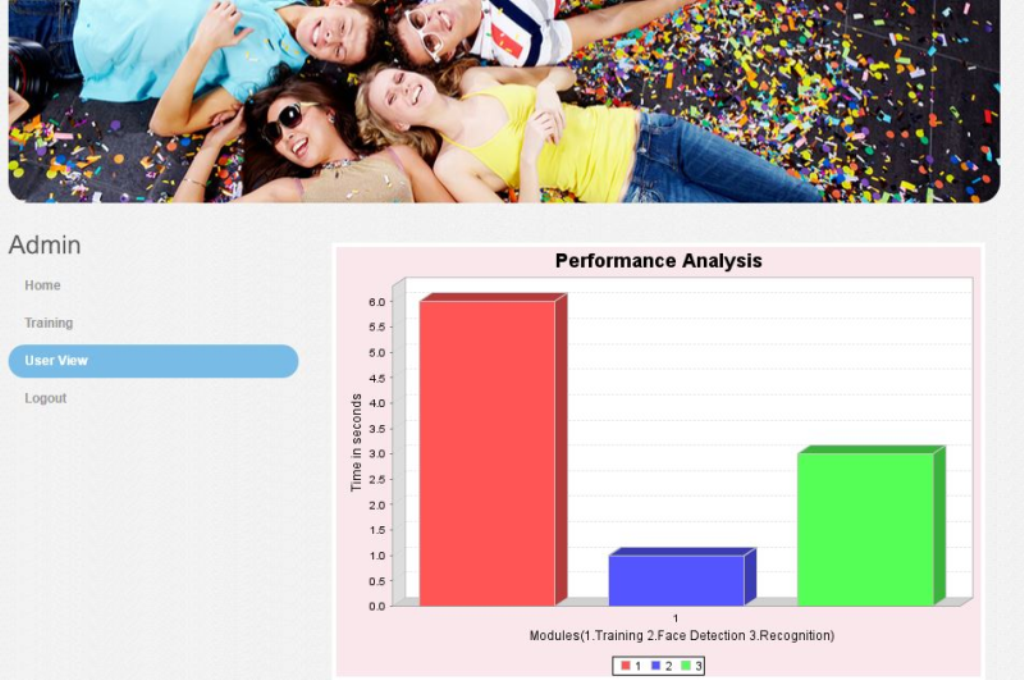
\includegraphics[width=\textwidth]{newperfomance.png}
           % \text{\scriptsize(ISO 9001:2008 Certified)}
            \caption[Performance Analysis Graph]{Performance analysis graph}
             \label{PerformanceAnalysis}
\end{center}
 \end{minipage}          
\end{figure}
\begin{table}[H]
\centering
\caption{Observation table for proposed system}
\label{routing}
\vspace{.5cm}
\begin{tabular}{|c|c|c|}
\hline
\textbf{SNO:} &\textbf{Modules}       &\textbf{Time taken(seconds)}  \\
\hline
1     &Training    &   7      \\
      
\hline
1     &FaceDetection    &   2      \\
      
\hline
4 &Face Recognition&2            \\
\hline
\end{tabular}
\end{table}
\clearpage


\clearpage











%%%%%%%%%%%%%%%%%%%%%%%[ CONCLUSION]%%%%%%%%%%%%%%%%%
%\addtocontents{toc}{\cftpagenumberson{chapter}}

\chapter[CONCLUSION]{\fontsize{16}{12}\selectfont CONCLUSION }

Photo sharing is one of the most popular features in online social networks such as Facebook. Lamentably, imprudent photograph posting may uncover security of people in a posted photograph. To control the security spillage, we proposed to empower people possibly in a photograph to give the consents before posting a co-photograph. We planned a security safeguarding FR framework to recognize people in a co-photograph. The proposed framework is highlighted with low calculation expense and privacy of the preparation set. Hypothetical examination and trials were directed to show adequacy and effectiveness of the proposed plan. We expect that our proposed plan be exceptionally helpful in ensuring clients' protection in photograph/picture sharing over online informal organizations.Our future work could be the way to move the proposed preparing plans to individual mists like Dropbox and/or icloud.Secured video sharing through online social networking will also be our future enhancement. 

 \newpage
 \thispagestyle{empty}
 
%\end{document}
%%%%%%%%%%%%%%%%%%%%%%%%%[ END OF CHAPTERS ]%%%%%%%%%%%%%%%%%%%%%%%%%%%%%%%%%%

\end{comment}